
\documentclass[xetex,professionalfont]{beamer}

\usepackage{amsmath}

\usepackage{mathtools}

\usepackage{amssymb}

\usepackage{xspace}

\usepackage{booktabs}

\usepackage{copyrightbox}


\usepackage{fontspec}
\setmonofont[Scale=0.7]{Droid Sans Mono} %

\usepackage[caption=false]{subfig}
\captionsetup{belowskip=0pt,aboveskip=0pt}

\usepackage{csquotes}


\usepackage[english]{babel}


\usepackage{tikz}
\usepackage{pgfplots}


\hypersetup{pdftitle={DLVC Introduction},pdfsubject={},pdfauthor={Christopher Pramerdorfer},colorlinks,urlcolor=tuwcvl_cvl_blue,linkcolor=tuwcvl_textlight}

\makeatletter\renewcommand{\CRB@setcopyrightfont}{\tiny\color{lightgray}}

\let\oldemph\emph
\renewcommand\emph[1]{\textcolor{tuwcvl_cvl_blue}{#1}}

\usefonttheme[onlymath]{serif}

\usetheme{dlvc}



\newcommand{\ie}{\mbox{i.e.}\xspace} %
\newcommand{\eg}{\mbox{e.g.}\xspace} %

\DeclareMathOperator*{\argmin}{arg\,min}
\DeclareMathOperator*{\argmax}{arg\,max}

\newcommand{\NN}{\mathbb{N}}
\newcommand{\ZZ}{\mathbb{Z}}
\newcommand{\QQ}{\mathbb{Q}}
\newcommand{\RR}{\mathbb{R}}

\renewcommand{\vec}[1]{\ensuremath{\mathbf{#1}}}

\newcommand{\va}{\vec{a}}
\newcommand{\vb}{\vec{b}}
\newcommand{\vc}{\vec{c}}
\newcommand{\ve}{\vec{e}}
\newcommand{\vr}{\vec{r}}
\newcommand{\vs}{\vec{s}}
\newcommand{\vt}{\vec{t}}
\newcommand{\vu}{\vec{u}}
\newcommand{\vv}{\vec{v}}
\newcommand{\vw}{\vec{w}}
\newcommand{\vx}{\vec{x}}
\newcommand{\vy}{\vec{y}}
\newcommand{\vz}{\vec{z}}

\makeatletter
\let\@@magyar@captionfix\relax
\makeatother


\title{Deep Learning for Visual Computing}
\subtitle{Motivation, Image Classification}
\author{Christopher Pramerdorfer}
\institute{Computer Vision Lab, TU Wien}

\begin{document}


\begin{frame}
\maketitle
\end{frame}


\begin{frame}
\frametitle{This Week in AI}
\framesubtitle{GPT-4}

\begin{center}
  \copyrightbox[b]
  {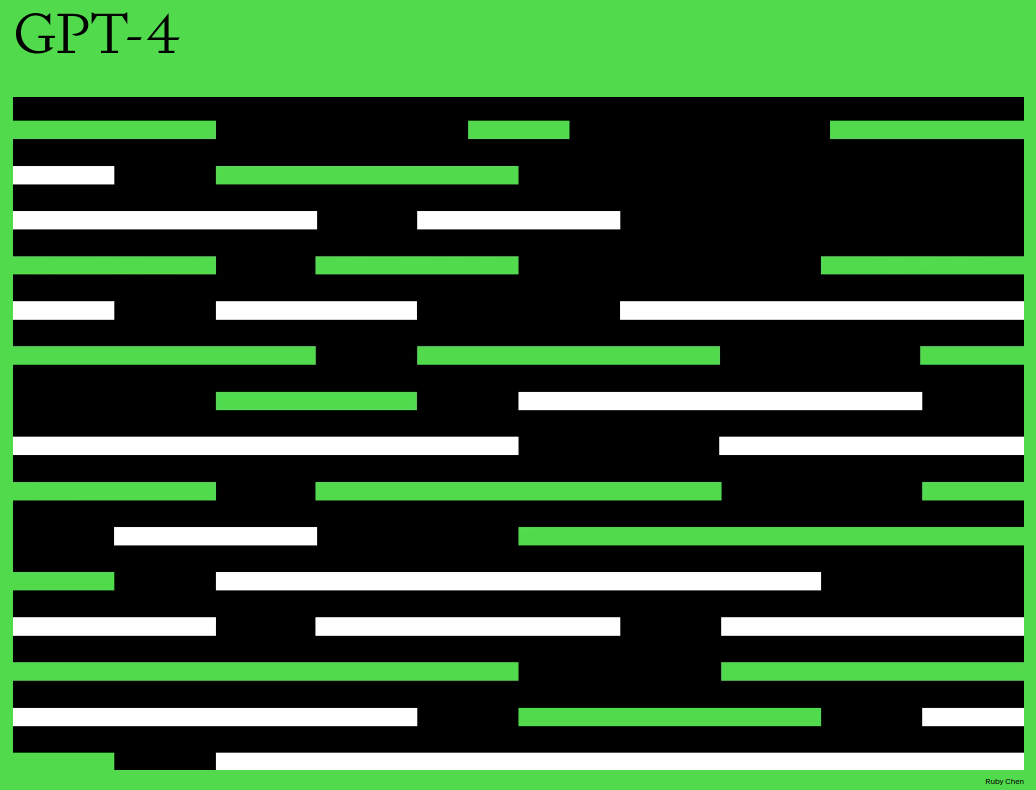
\includegraphics[width=7cm]{images/gpt4}}
  {\centering Image from \href{https://chat.openai.com/chat}{OpenAI}}
\end{center}

\end{frame}


\begin{frame}
\frametitle{Topics}

Deep learning
\begin{itemize}
    \item Motivation
    \item Primer
\end{itemize}

\bigskip

Image classification
\begin{itemize}
    \item Challenges
    \item Datasets
    \item Manual approach
\end{itemize}

\end{frame}


\begin{frame}
\frametitle{Motivation for Deep Learning}

Course is called Deep Learning for \emph{Visual Computing}
\begin{itemize}
    \item Very generic term (includes computer graphics etc.) %
\end{itemize}

\bigskip

We'll focus on \emph{computer vision}
\begin{itemize}
    \item Make computers gain \emph{high-level} understanding of images
    \item Goal is human-like understanding %
\end{itemize}

\bigskip

\emph{Deep learning} has revolutionized this field
\begin{itemize}
    \item Reason for the current AI hype %
\end{itemize}

\end{frame}


\begin{frame}
\frametitle{Motivation for Deep Learning}
\framesubtitle{Image Classification}

\begin{center}
\enquote{What thing is shown in this image?}
\end{center}

\smallskip

\begin{center}
    \copyrightbox[b]
    {
    \begin{tikzpicture}
        \node[anchor=south west,inner sep=0] (image) at (0,0) {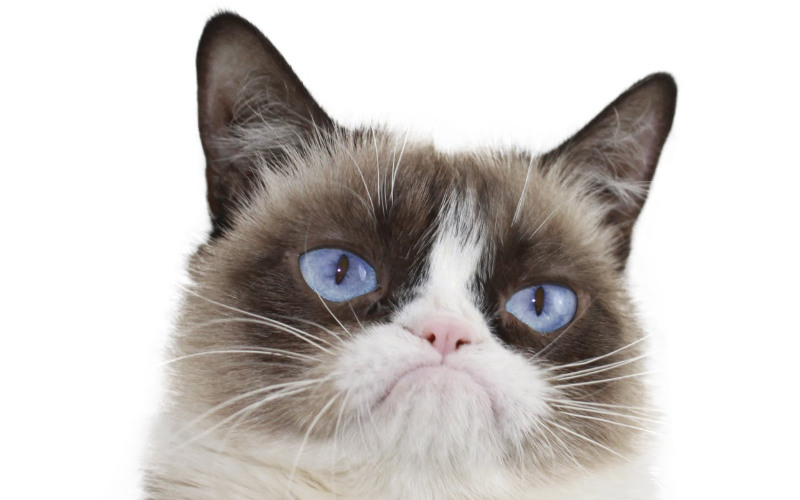
\includegraphics[width=5cm]{images/grumpy-cat.jpg}};
        \node[tuwcvl_inf_red] at (5.3, 1) {$\quad\Rightarrow\quad$ cat};
    \end{tikzpicture}
    }
    {\centering Image from youtube.com}
\end{center}

\end{frame}


\begin{frame}
\frametitle{Motivation for Deep Learning}
\framesubtitle{Image Classification}

ImageNet benchmark performance over time
\begin{itemize}
    \item 100k test images of 1000 classes
\end{itemize}

\medskip

\begin{center}
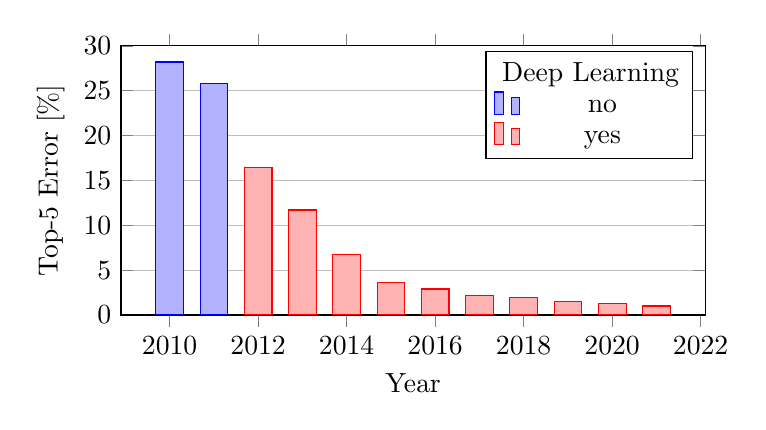
\begin{tikzpicture}
\begin{axis}[
    ybar,
    x tick label style={/pgf/number format/1000 sep=},
    xlabel=Year,
    ylabel={Top-5 Error [\%]}, %
    ylabel near ticks,
    ymajorgrids = true,
    ymin = 0,
    ymax = 30,
    width = 9cm,
    height = 5cm,
    ytick = {0,5,10,15,20,25,30}
]
\addlegendimage{empty legend}
\addplot+ [bar shift = 0pt] coordinates {(2010,28.2) (2011,25.8)};
\addplot+ [bar shift = 0pt] coordinates {(2012,16.4) (2013,11.7) (2014,6.7) (2015,3.6) (2016,2.9) (2017,2.2) (2018,1.9) (2019,1.5) (2020,1.3) (2021,1.0)};
\addlegendentry{\hspace{-.3cm}Deep Learning}
\addlegendentry{no}
\addlegendentry{yes}
\end{axis}
\end{tikzpicture}
\end{center}

\end{frame}


\begin{frame}
\frametitle{Motivation for Deep Learning}
\framesubtitle{Object Detection}

\begin{center}
\enquote{Detect objects of interest} %
\end{center}

\smallskip

\begin{center}
    {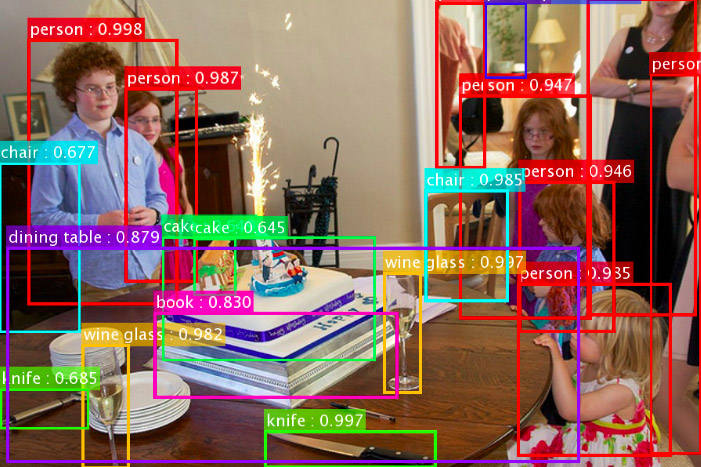
\includegraphics[width=7cm]{images/rrcnn-coco}}
\end{center}

\end{frame}


\begin{frame}
\frametitle{Motivation for Deep Learning}
\framesubtitle{Instance Segmentation}

\begin{center}
\enquote{Delineate objects of interest} %
\end{center}

\smallskip

\begin{center}
    \copyrightbox[b]
    {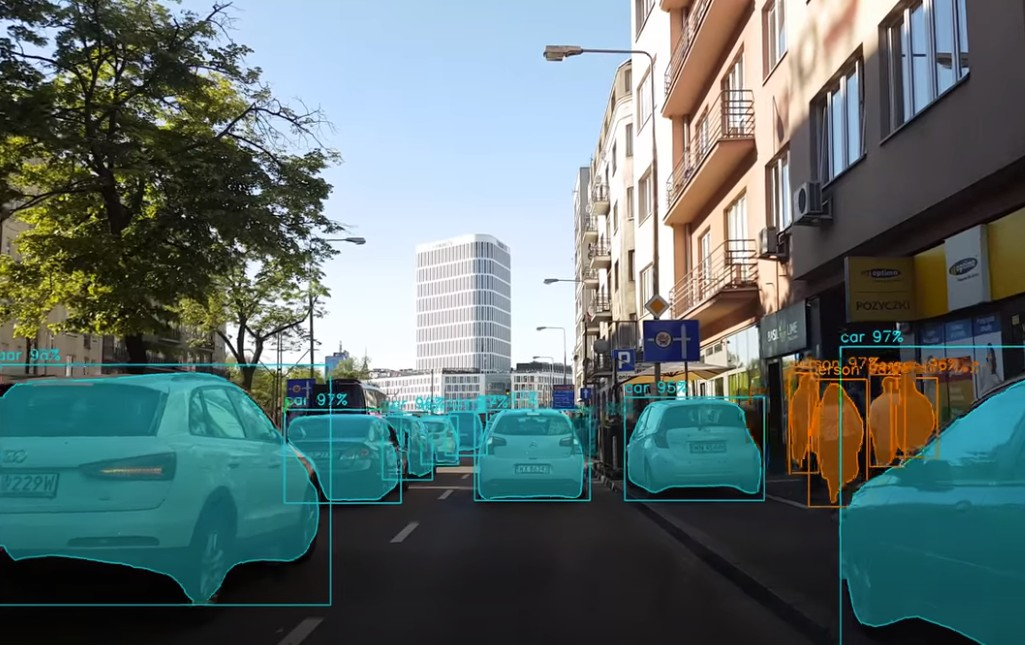
\includegraphics[width=7cm]{images/mask-rcnn-traffic}}
    {\centering\href{https://www.youtube.com/watch?v=OOT3UIXZztE}{link}} %
\end{center}

\end{frame}


\begin{frame}
\frametitle{Motivation for Deep Learning}
\framesubtitle{Pose Estimation}

\begin{center}
    \enquote{Estimate people's poses} %
\end{center}

\smallskip


\begin{center}
    \copyrightbox[b]
    {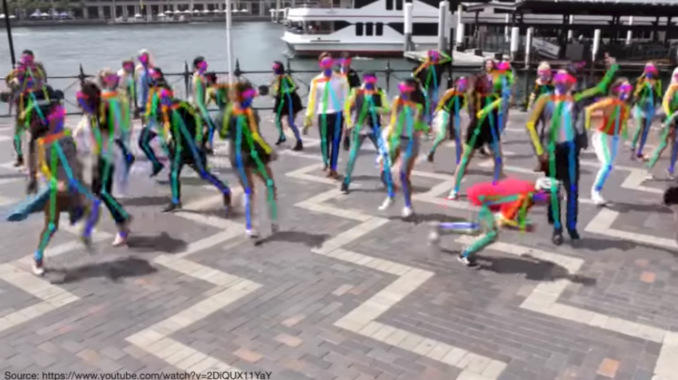
\includegraphics[width=7cm]{images/pose}}
    {\centering\href{https://www.youtube.com/watch?v=pW6nZXeWlGM}{link}}
\end{center}

\end{frame}


\begin{frame}
\frametitle{Motivation for Deep Learning}
\framesubtitle{Image Synthesis}

\begin{center}
    \enquote{Be an artist} 
\end{center}



\smallskip

\begin{center}
    \copyrightbox[b]
    {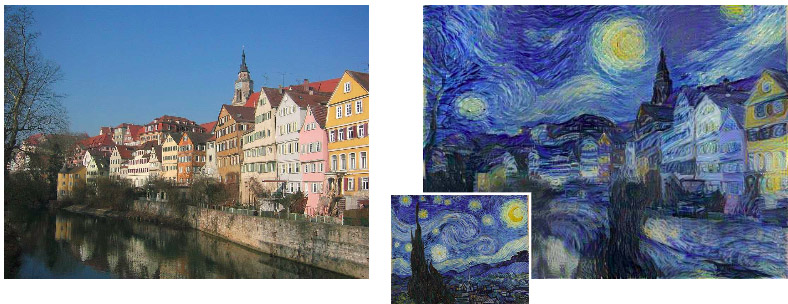
\includegraphics[width=10cm]{images/style}}
    {\centering\href{http://genekogan.com/works/style-transfer/}{link}}
\end{center}

\end{frame}


\begin{frame}
\frametitle{Motivation for Deep Learning}
\framesubtitle{Image Synthesis}

\begin{center}
    \enquote{Be an artist} (really)
\end{center}

\smallskip

\begin{center}
    \copyrightbox[b]
    {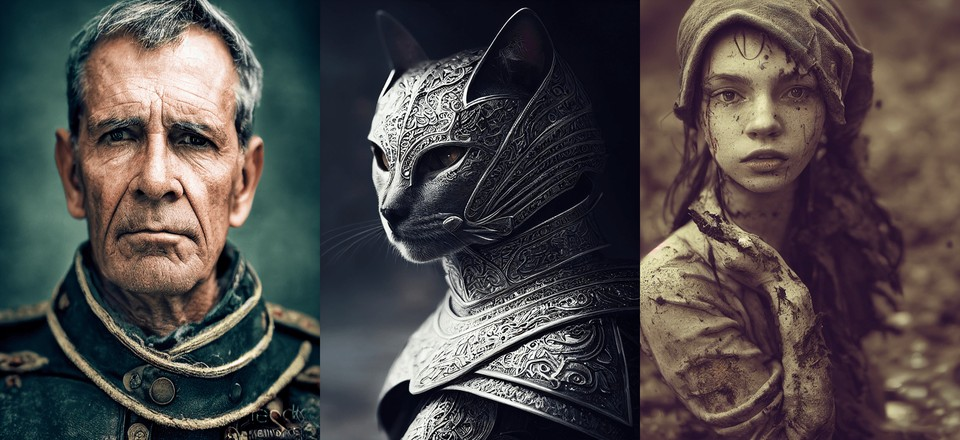
\includegraphics[width=9cm]{images/stable-diffusion}}
    {\centering midjourney.com}
\end{center}

\end{frame}


\begin{frame}
\frametitle{Motivation for Deep Learning}
\framesubtitle{Image Synthesis}

\begin{center}
\enquote{Be a 3D artist}
\end{center}

\smallskip

\begin{center}
    \copyrightbox[b]
    {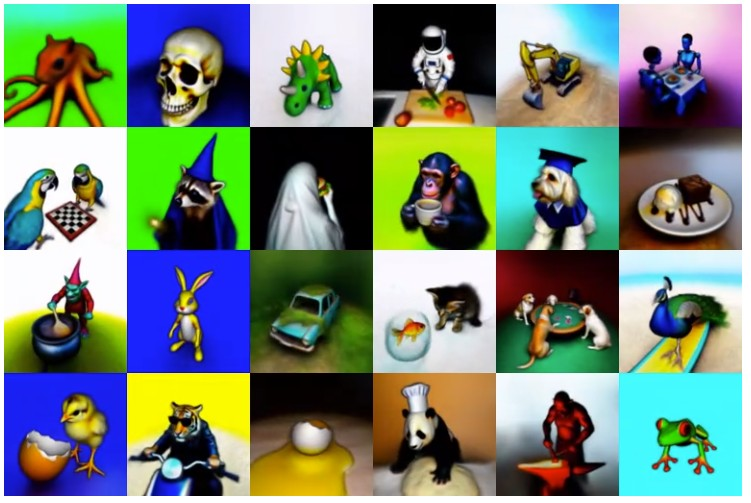
\includegraphics[width=6.5cm]{images/dreamfusion}}
    {\centering\href{https://dreamfusion3d.github.io}{link}}
\end{center}
    
\end{frame}


\begin{frame}
\frametitle{Motivation for Deep Learning}
\framesubtitle{Image Synthesis}

\begin{center}
\enquote{Generate videos that look real}
\end{center}

\smallskip

\begin{center}
    \copyrightbox[b]
    {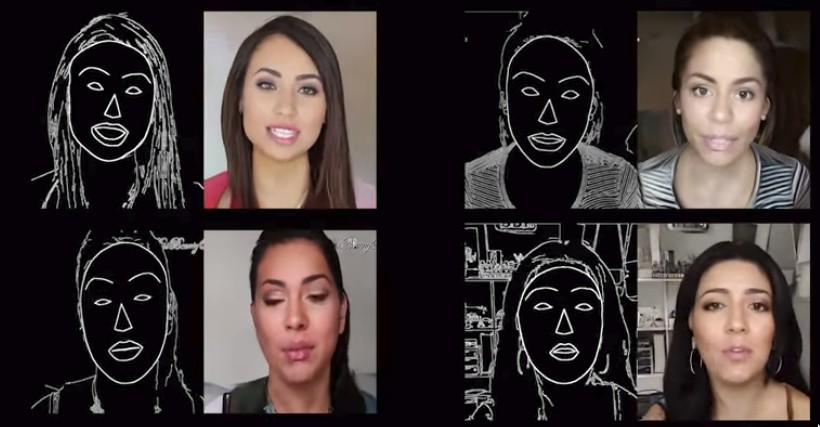
\includegraphics[width=7cm]{images/facegen}}
    {\centering\href{https://www.youtube.com/watch?v=GrP_aOSXt5U}{link}} %
\end{center}

\end{frame}


\begin{frame}
\frametitle{Motivation for Deep Learning}
\framesubtitle{Image Synthesis}

\begin{center}
\enquote{Generate videos that look real} (danger!)
\end{center}

\smallskip

\begin{center}
    \copyrightbox[b]
    {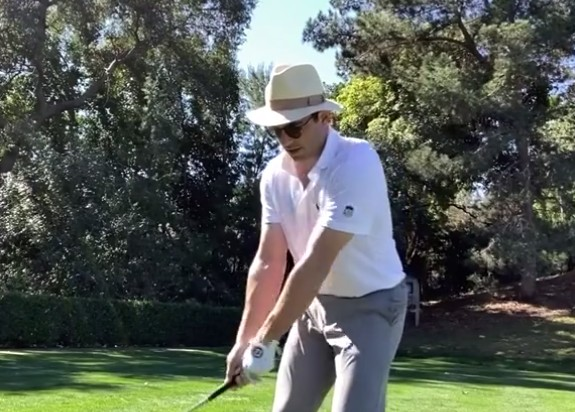
\includegraphics[width=6cm]{images/deep-fake}}
    {\centering\href{https://www.tiktok.com/@deeptomcruise/video/6932166297996233989?is_copy_url=1&is_from_webapp=v1}{link}}
\end{center}
    
\end{frame}


\begin{frame}
\frametitle{Motivation for Deep Learning}
\framesubtitle{Image Understanding}

\begin{center}
    \enquote{Explain what's going on in an image} %
\end{center}

\smallskip

\begin{center}
    \copyrightbox[b]
    {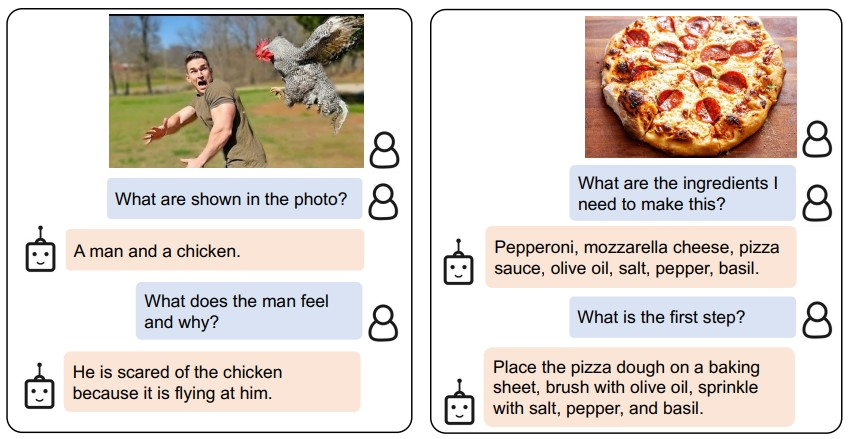
\includegraphics[width=9cm]{images/blip-2}}
    {\centering\href{https://arxiv.org/pdf/2301.12597.pdf}{paper}}
\end{center}
    
\end{frame}


\begin{frame}
\frametitle{Motivation for Deep Learning}

All these examples are based on deep learning
\begin{itemize}
    \item Would be impossible otherwise (at this quality)
    \item We will take a closer look throughout the lecture
\end{itemize}

\bigskip

Deep learning is state of the art
\begin{itemize}
    \item In virtually any computer vision task
    \item In most other fields as well (\eg speech recognition)
\end{itemize}

\bigskip

So knowledge of deep learning is essential %

\end{frame}


{
\setbeamertemplate{footline}{}
\begin{frame}

\begin{tikzpicture}[remember picture,overlay]
\fill[white] (current page.north west) rectangle (current page.south east);
\end{tikzpicture}

\begin{center}
\textcolor[rgb]{0.9,0.9,0.9}{blank page}
\end{center}

\end{frame}
}


\begin{frame}
\frametitle{Deep Learning Primer}

Deep learning is not magic %
\begin{itemize}
    \item Implemented using neural networks
    \item With neurons that are adapted for image data
    \item And arranged in many layers (hence \enquote{deep})
\end{itemize}

\bigskip

Machine learning concepts still apply %
\begin{itemize}
    \item Parametric models
    \item Loss functions \& iterative optimization
    \item Overfitting, regularization
\end{itemize}

\end{frame}


\begin{frame}
\frametitle{Deep Learning Primer}

The power of deep learning comes from
\begin{itemize}
    \item Hierarchical local feature transformations %
    \item That are learned using large amounts of data %
\end{itemize}

\bigskip

Key ingredients needed
\begin{itemize}
    \item Large datasets
    \item Lots of processing power
\end{itemize}

\end{frame}


\begin{frame}
\frametitle{Deep Learning Primer}

Learn high-level concepts from lower-level ones %

\medskip

\begin{center}
    \copyrightbox[b]
    {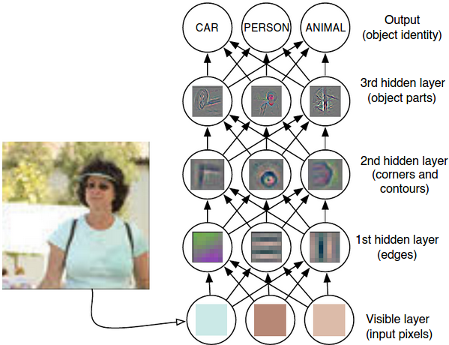
\includegraphics[width=6cm]{images/dl-layers}}
    {\centering Image from deeplearningbook.org}
\end{center}

\end{frame}


\begin{frame}
\frametitle{Deep Learning Primer}

Deep learning is $30+$ years old %
\begin{itemize}
    \item But data and processing power were limited until recently %
\end{itemize}

\medskip

\begin{center}
    \copyrightbox[b]
    {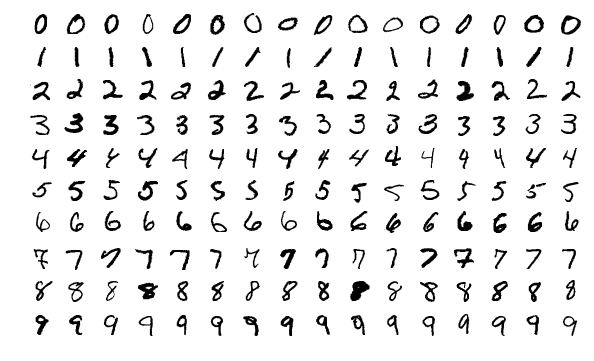
\includegraphics[width=6cm]{images/mnist}}
    {\centering Image from Wikipedia}
\end{center}

\end{frame}


\begin{frame}
\frametitle{Deep Learning Primer}

Nowadays deep learning is a billion dollar business
\begin{itemize}
    \item Big tech companies embraced it years ago
    \item We interact with deep learning daily (\eg phones, cars) %
\end{itemize}

\medskip

\begin{center}
    \copyrightbox[b]
    {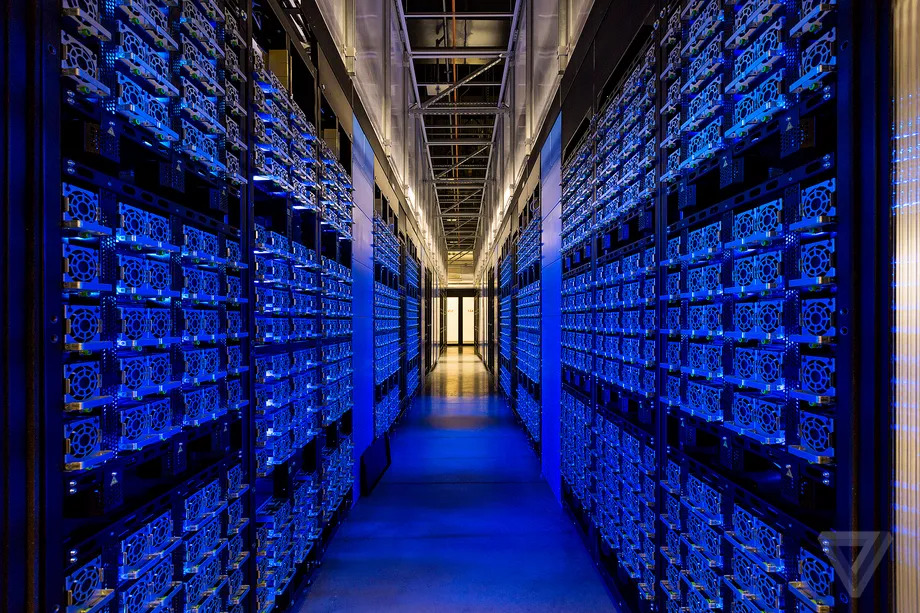
\includegraphics[width=6cm]{images/datacenter}} %
    {\centering\href{https://www.theverge.com/2022/1/24/22898651/meta-artificial-intelligence-ai-supercomputer-rsc-2022}{link}}
\end{center}

\end{frame}


\begin{frame}
\frametitle{Deep Learning Primer}

Deep learning has become accessible
\begin{itemize}
    \item The software used by Google, Meta etc. is open source
    \item Runs on your PC and even on your phone
    \item Cloud services available (\eg Google Colab) %
\end{itemize}

\medskip

\begin{center}
    \copyrightbox[b]
    {
\includegraphics[width=4cm]{images/pytorch-logo}}
    {\centering\href{https://pytorch.org/}{link}}
\end{center}

\end{frame}


{
\setbeamertemplate{footline}{}
\begin{frame}

\begin{tikzpicture}[remember picture,overlay]
\fill[white] (current page.north west) rectangle (current page.south east);
\end{tikzpicture}

\begin{center}
\textcolor[rgb]{0.9,0.9,0.9}{blank page}
\end{center}

\end{frame}
}


\begin{frame}
\frametitle{Image Classification}

Fundamental computer vision task

\bigskip

Definition
\begin{itemize}
    \item Given a set of \emph{class labels} (e.g. \{bird, cat, dog\})
    \item Which class does the given image belong to?
\end{itemize}

\begin{center}
    \copyrightbox[b]
    {
    \begin{tikzpicture}
        \node[anchor=south west,inner sep=0] (image) at (0,0) {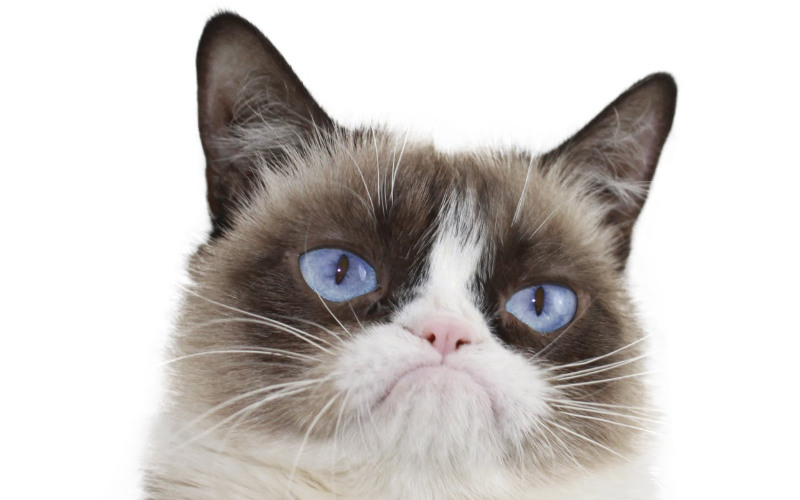
\includegraphics[width=4cm]{images/grumpy-cat.jpg}};
        \node[tuwcvl_inf_red] at (4.3, 1) {$\quad\Rightarrow\quad$ cat};
    \end{tikzpicture}
    }
    {\centering Image from youtube.com}
\end{center}

\end{frame}


\begin{frame}
\frametitle{Image Classification}

Image belongs to exactly one class in the set
\begin{itemize}
    \item Comparatively easy task (but still challenging)
    \item On many datasets deep learning outperforms humans
\end{itemize}

\bigskip

Simple problem formulation
\begin{itemize}
    \item Great for learning deep learning basics
    \item Why we will stick to classification for now
\end{itemize}

\end{frame}


\begin{frame}
\frametitle{Image Classification}
\framesubtitle{Challenges -- Pose and Viewpoint}

\begin{center}
    \copyrightbox[b]
    {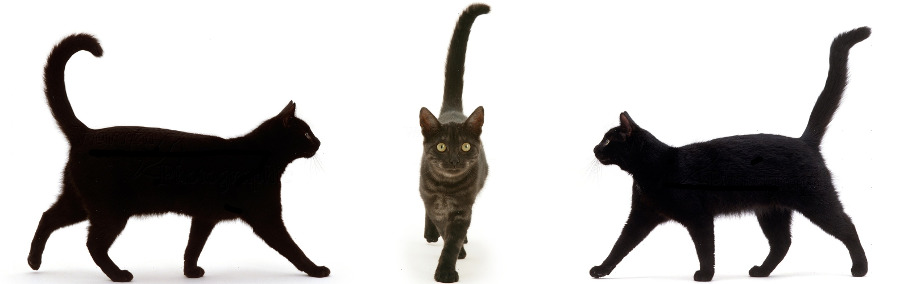
\includegraphics[width=10cm]{images/cat-viewpoints.jpg}}
    {\centering Image adapted from warrenphotographic.co.uk} %
\end{center}

\end{frame}


\begin{frame}
\frametitle{Image Classification}
\framesubtitle{Challenges -- Illumination}

\begin{center}
    \copyrightbox[b]
    {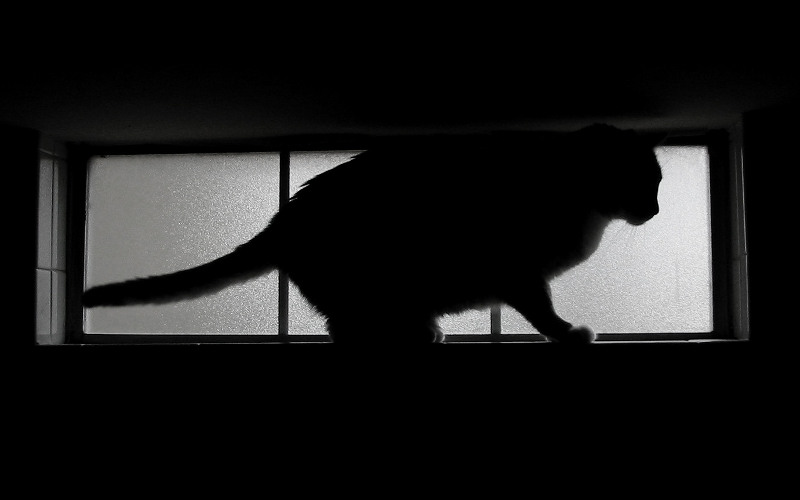
\includegraphics[width=8cm]{images/cat-darkness.jpg}}
    {\centering Image from studioddt.com}
\end{center}

\end{frame}


\begin{frame}
\frametitle{Image Classification}
\framesubtitle{Challenges -- Deformation}

\begin{center}
    \copyrightbox[b]
    {
\includegraphics[width=11cm]{images/cat-deformation.jpg}}
    {\centering Image from \href{http://cs231n.github.io/}{cs231n.github.io}} %
\end{center}

\end{frame}


\begin{frame}
\frametitle{Image Classification}
\framesubtitle{Challenges -- Occlusion}

\begin{center}
    \copyrightbox[b]
    {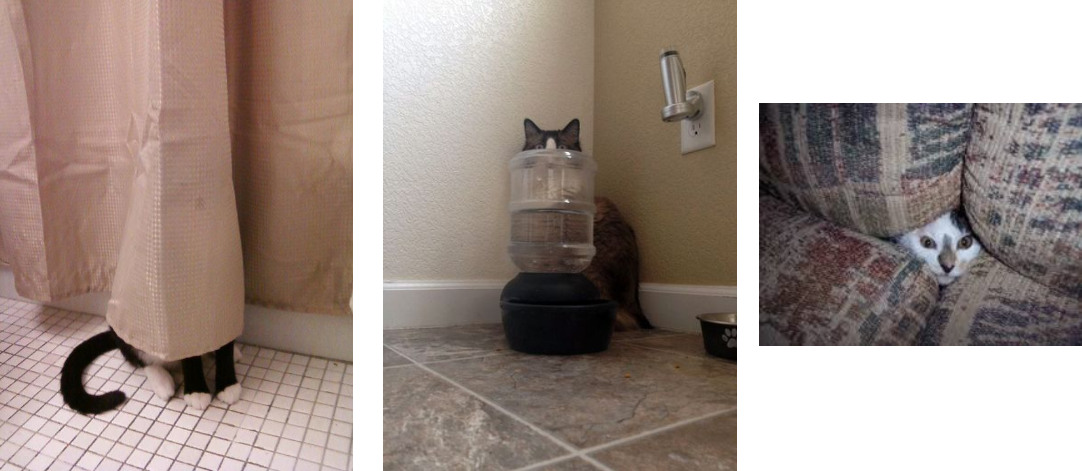
\includegraphics[width=10cm]{images/cat-occlusion.jpg}}
    {\centering Image from \href{http://cs231n.github.io/}{cs231n.github.io}} %
\end{center}

\end{frame}


\begin{frame}
\frametitle{Image Classification}
\framesubtitle{Challenges -- Background}

\begin{center}
    \copyrightbox[b]
    {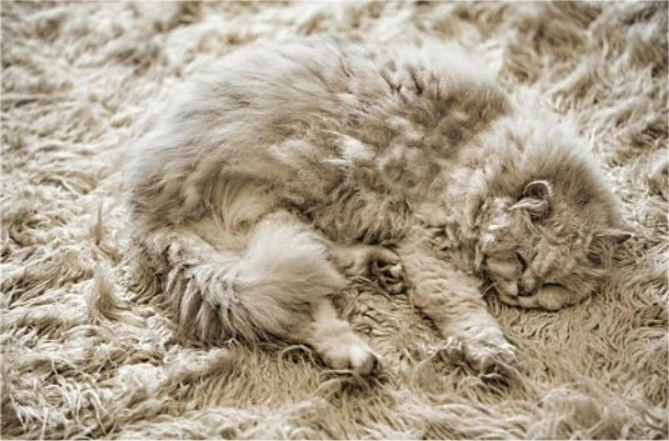
\includegraphics[width=8cm]{images/cat-background.jpg}}
    {\centering Image from \href{http://cs231n.github.io/}{cs231n.github.io}} %
\end{center}

\end{frame}


\begin{frame}
\frametitle{Image Classification}
\framesubtitle{Challenges -- Intraclass Variation}

\begin{center}
    \copyrightbox[b]
    {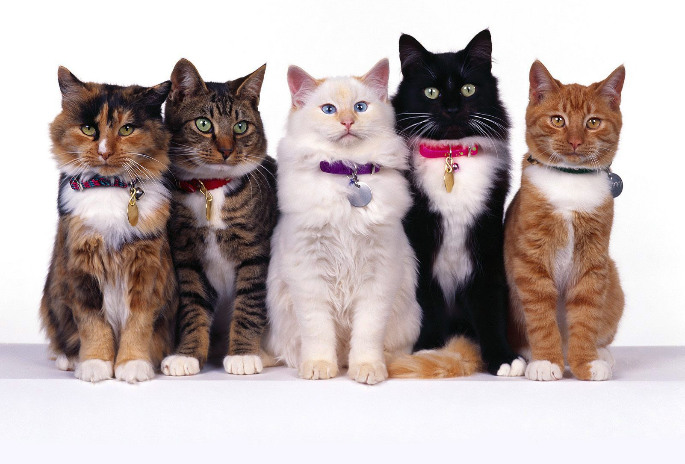
\includegraphics[width=8cm]{images/cat-class-variation.jpg}} %
    {\centering Image from \href{http://cs231n.github.io/}{cs231n.github.io}}
\end{center}

\end{frame}


\begin{frame}
\frametitle{Image Classification}
\framesubtitle{Datasets}

A good classifier must cope with these challenges
\begin{itemize}
    \item To verify this we need a representative dataset %
    \item Such datasets are usually large
\end{itemize}

\bigskip

If we employ \emph{machine learning} we also need training data
\begin{itemize}
    \item Datasets must be disjoint (so need even more data) %
    \item Deep learning requires lots of data
\end{itemize}

\end{frame}


\begin{frame}
\frametitle{Image Classification}
\framesubtitle{Datasets}

Dataset acquisition takes lots of effort
\begin{itemize}
    \item Collect many (thousands or more) of images
    \item Assign class labels to enable automatic training and testing
\end{itemize}

\bigskip

Data acquisition and processing is central in deep learning
\begin{itemize}
    \item Often the most time-consuming task
    \item Usually main bottleneck for performance
\end{itemize}

\bigskip

Thankfully many public datasets are available

\end{frame}


\begin{frame}
\frametitle{Image Classification}
\framesubtitle{Datasets -- CIFAR-10}

10 classes, 60k images

\bigskip

\begin{center}
    \copyrightbox[b]
    {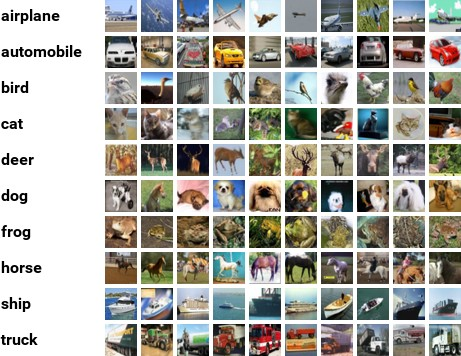
\includegraphics[width=6cm]{images/cifar10.jpg}}
    {\centering Image from \href{https://www.cs.toronto.edu/~kriz/cifar.html}{cs.toronto.edu}}
\end{center}

\end{frame}


\begin{frame}
\frametitle{Image Classification}
\framesubtitle{Datasets -- ImageNet}

20k classes, 14m images %
\begin{itemize}
    \item One of main drivers for deep learning performance %
\end{itemize}

\bigskip

\begin{center}
    \copyrightbox[b]
    {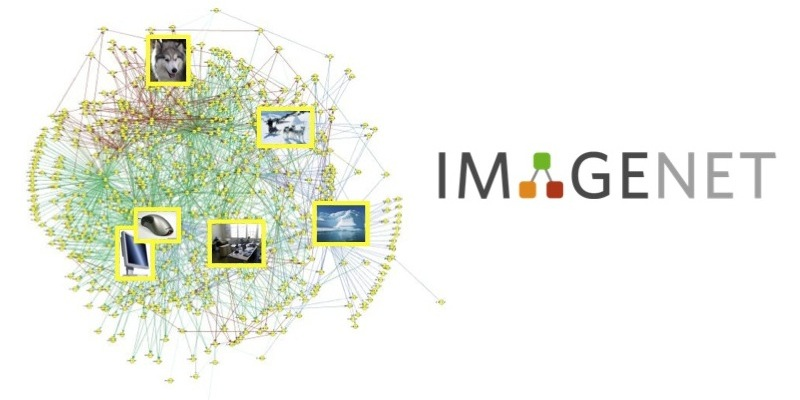
\includegraphics[width=7cm]{images/imagenet.jpg}}
    {\centering Image from umich.edu}
\end{center}

\end{frame}


\begin{frame}
\frametitle{Image Classification}
\framesubtitle{Datasets -- COCO}

300k images, labels for classification, detection, segmentation, ... %

\bigskip

\begin{center}
    \copyrightbox[b]
    {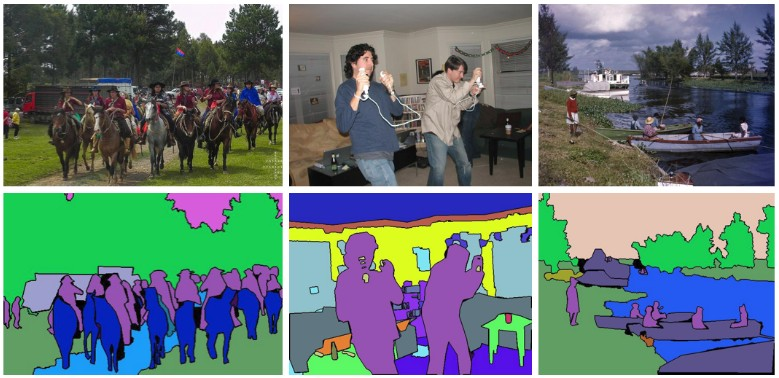
\includegraphics[width=8cm]{images/coco.jpg}}
    {\centering Image from \href{http://cocodataset.org}{cocodataset.org}}
\end{center}

\end{frame}


\begin{frame}
\frametitle{Image Classification}

Let's build an image classifier
\begin{itemize}
    \item Should support the classes \{dog, cat\}
    \item Using the CIFAR-10 dataset
\end{itemize}

\bigskip

\begin{center}
    \copyrightbox[b]
    {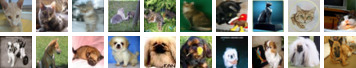
\includegraphics[width=10cm]{images/cifar10-catsdogs.jpg}}
    {\centering Image from cs.toronto.edu}
\end{center}

\end{frame}


\begin{frame}
\frametitle{Image Classification}

How can we write an algorithm for this purpose? %

\bigskip

\begin{center}
    \copyrightbox[b]
    {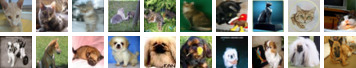
\includegraphics[width=10cm]{images/cifar10-catsdogs.jpg}}
    {\centering Image from cs.toronto.edu}
\end{center}

\end{frame}


\begin{frame}
\frametitle{Image Classification}

We cannot!
\begin{itemize}
    \item No obvious unique and reliable \emph{features} %
    \item Not clear how to represent and use them
\end{itemize}

\bigskip

\begin{center}
    \copyrightbox[b]
    {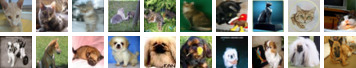
\includegraphics[width=10cm]{images/cifar10-catsdogs.jpg}}
    {\centering Image from cs.toronto.edu}
\end{center}

\end{frame}


\begin{frame}
\frametitle{Image Classification}

We humans are incredible image classifiers

\bigskip

But we cannot describe formally how we do so
\begin{itemize}
    \item Thus the standard \texttt{if \{\} else \{\}} approach fails
\end{itemize}

\bigskip

This applies to most vision problems
\begin{itemize}
    \item Reason we need machine and deep learning
\end{itemize}

\end{frame}

\end{document}
